\subsubsection{Funktionsweise}

Bei der Bilderzeugung, ausgehend von Szenen, welche viel Geometrie beinhalten bzw. bei Szenen 
die generelle BRDF's verwenden eignet sich der \nameref{ch:Content1:sec:PathTracer}.
Der \nameref{ch:Content1:sec:PathTracer} ist in Hinsicht der Beleuchtung komplett. Deshalb lässt sich damit
\textit{Global Illumination} erreichen. Der hier verwendete \nameref{ch:Content1:sec:PathTracer} in 
\cite{Benty18} verwendet eine klassische Umsetzung.\par
Der Path Tracer beruht auf Erkenntnisse der Lösung der allgemeinen Rendergleichung.\ref{eq:kajiya}

\begin{equation}\label{eq:kajiya}
    I(x,{x}^{'}) = g(x,{x}^{'}) * \biggl[\epsilon(x,{x}^{'}) + 
    \int_{S}^{} \rho(x,{x}^{'},{x}^{''})
    I({x}^{'},{x}^{''}d{x}^{''})\biggr] 
\end{equation}

Sie beschreibt den Energietransport \textit{I} von einem Punkt ${x}^{'}$
zu einem Punkt x. Dabei ist ein maßgebender Faktor der Geometrieterm \textit{g},
der die relative Lage der beiden Punkte zueinander im Raum beschreibt.
Ein weiterer Faktor ist die Abstrahlung \textit{$\epsilon$} von ${x}^{'}$ nach x. 
Beeinflusst wird der Energiefluss auch durch
die bidirektionale Verteilungsfunktion \textit{$\rho$}, welche Aufschluss über
das einfallende Licht von einem Punkt ${x}^{''}$ über ${x}^{'}$ zu x gibt.\par
Die Schlussfolgerung aus dieser Gleichung \ref{eq:kajiya} ist: Die transportierte
Intensität von einem Licht zu einem Anderen ist die Summe des ausgestrahlten Lichts 
und das ausgestrahlte Licht zu x von allen anderen Oberflächen.

Ausgehend von der Rendergleichung \ref{eq:kajiya} lässt sich
die vollständige Transportgleichung\ref{eq:vollstaendige Transportgleichung} des \nameref{ch:Content1:sec:PathTracer}
beschreiben.
Wie in \cite{marschner2009fundamentals} beschrieben wird ausgehend von der vollständigen Transportgleichung
\ref{eq:vollstaendige Transportgleichung}

\begin{equation}\label{eq:vollstaendige Transportgleichung}
    L_s(k_0) = L_e(k_0) + \int_{all(k_i)}^{} \rho(k_i, k_0)*L_f(k_i)*cos(\theta_i)d\theta_i
\end{equation}

der vollständige Lichttransport beschrieben. Man kann deutlich die Ähnlichkeit
zu \ref{eq:kajiya} erkennen. Wir haben den Emissionsterm, die relative Lage der 
Punkte zueinander und die bidirektionale Verteilungsfunktion welche den Energietransport
beeinflussen.

\begin{figure}[H]
    \centering
    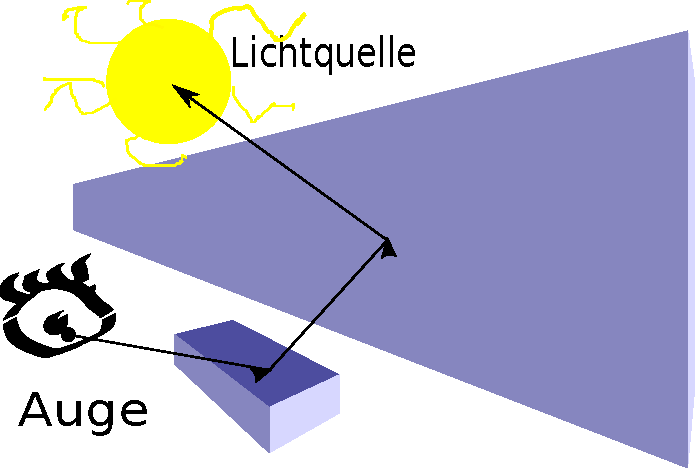
\includegraphics[width=0.7\linewidth]{content/PathTracer/Bilder/Grundkonzept_path_tracing.pdf}
    \label{pic::PathTracingGrundkonzept}
    \caption{Grundkonzept path tracer}
\end{figure}

\subsubsection{Monte-Carlo-Integration}
Mit der Monte Carlo Integration approximieren wir die Rendergleichung.\par 
Bei gegebener Funktion \textit{f }:\textit{ S}$\rightarrow \mathbb{R}$ und der 
Wahrscheinlichkeitsdichtefunktion $x \sim p$
\cite{KK02}
\cite{caflisch_1998}
Bildraum Fehler Randomisierung
\label{pic:MonteCarloIntegration}
\begin{equation}\label{eq:montcarlo}
    \int_{x\in S} g(x) d\mu \simeq \frac{1}{N}*\sum_{i=1}^{N}\frac{g(x_i)}{p(x_i)}
\end{equation}

\begin{figure}[H]\label{pic:WeissesRauschenTracer}
    \centering
    \begin{minipage}[t]{0.45\linewidth}
        \centering
        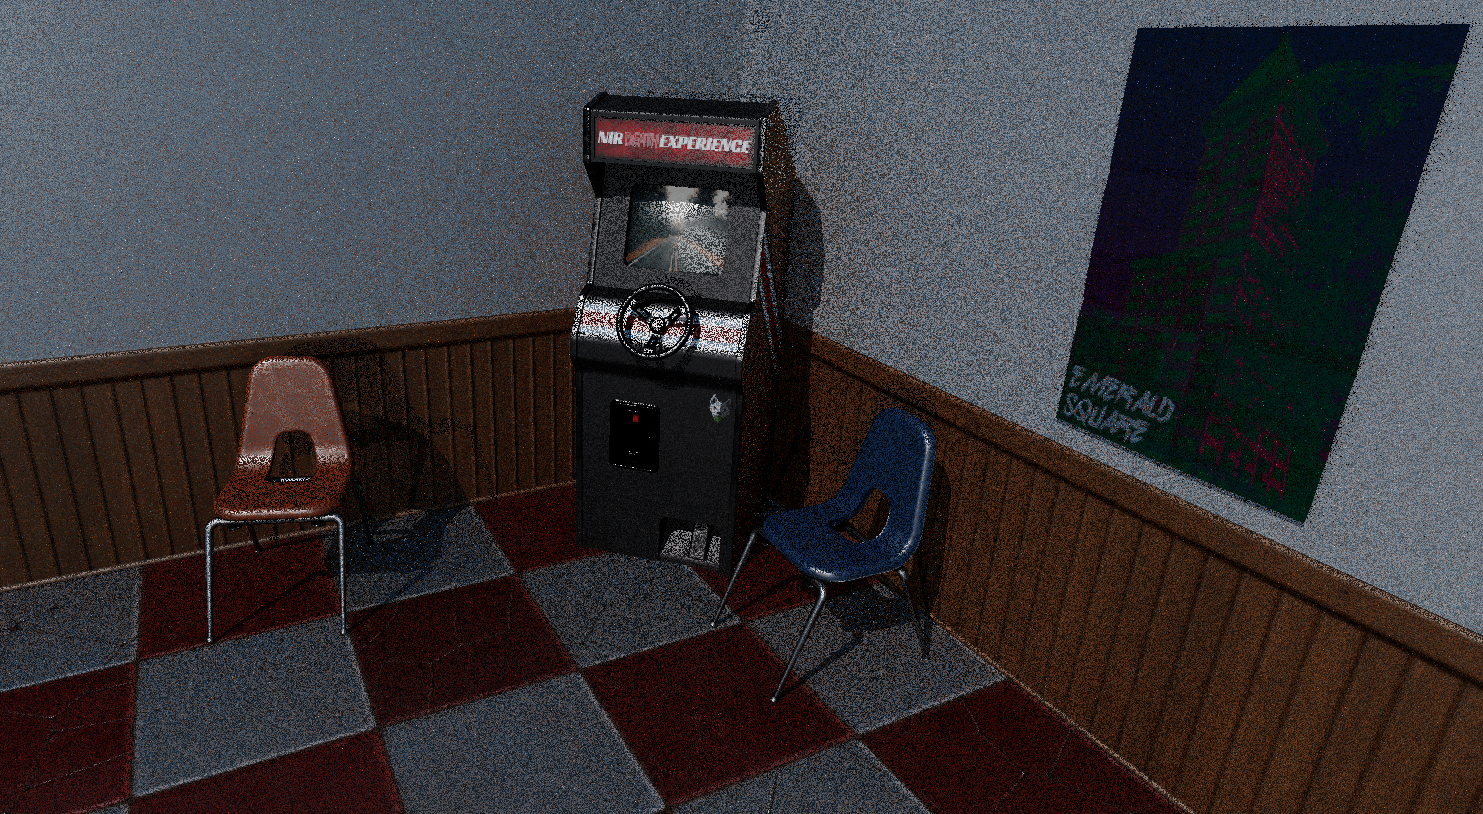
\includegraphics[width=\linewidth]{content/PathTracer/Bilder/WeissesRauschenSzene.png}
        \caption{Szene mit Weißem Rauschen}
    \end{minipage}
    \hfill
    \begin{minipage}[t]{0.45\linewidth}
        \centering
        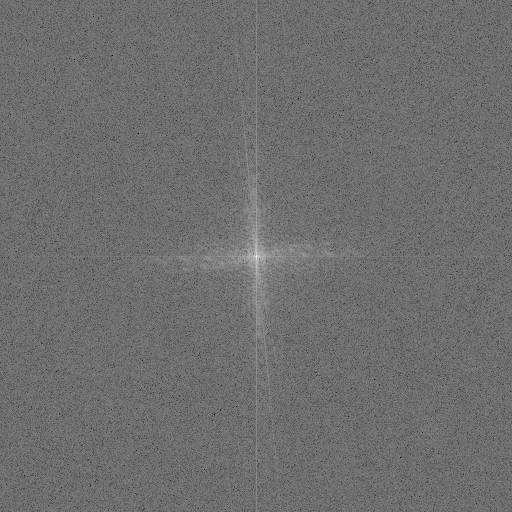
\includegraphics[width=\linewidth]{content/PathTracer/Bilder/FFT_Ausschnitt2.png}
        \caption{FFT des Ausschnitts}
    \end{minipage}
\end{figure}

\subsubsection{DirectX Raytracing}
Für besseres Verständnis möchte ich hier eine Einführung in das Path Tracing\cite{Benty18} mit Hilfe der
neuen DirectX-Schnittstelle geben.
\begin{figure}[H]
    \centering
    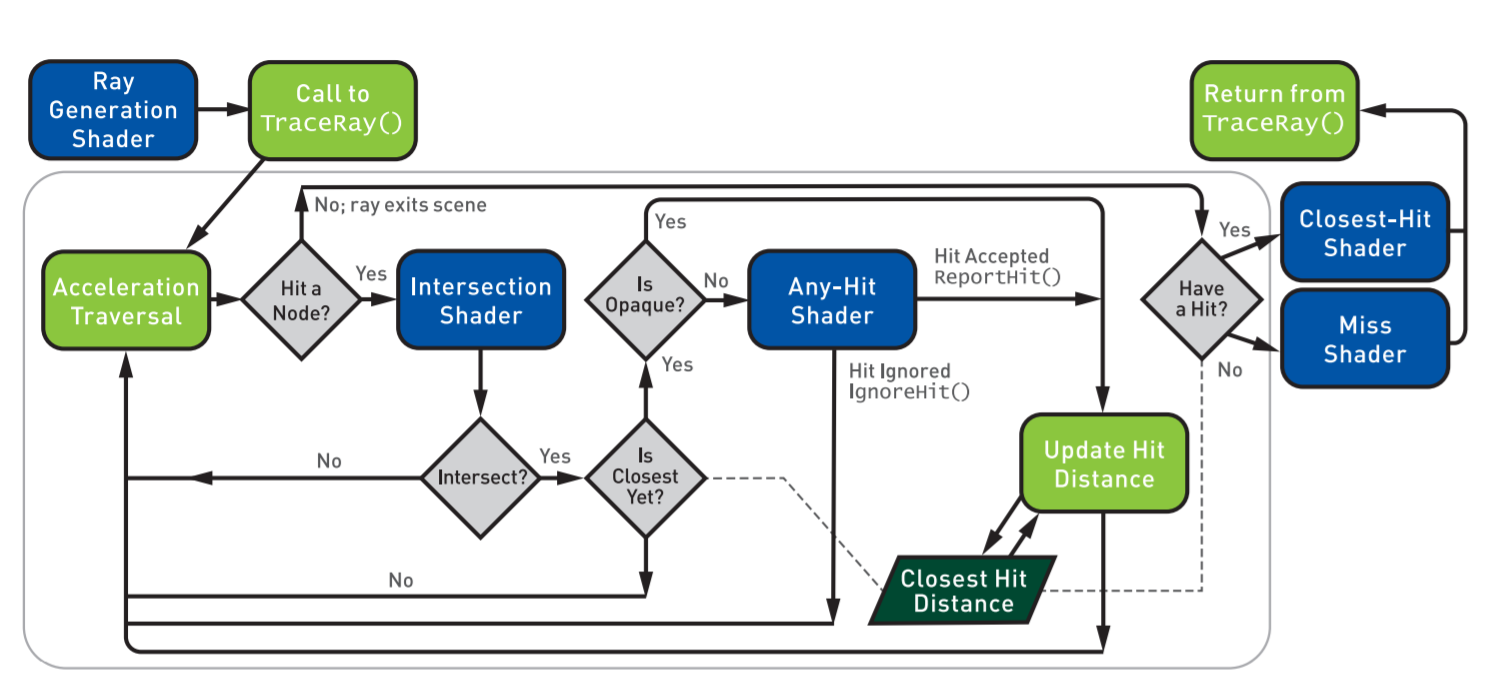
\includegraphics[width=\linewidth]{content/PathTracer/Bilder/DirectXRaytracingPipeline.png}
    \label{pic::DirectXRaytracingPipeline}
    \caption{DirectX Raytracing Pipeline aus \cite{Haines2019}}
\end{figure}

In der obigen Übersicht lässt sich der Start der neuen Pipeline erkennen, der \textbf{Ray Generation
shader}. Von hier aus werden Rays gestartet \textbf{TraceRay()}.
\textbf{Intersection shader} führt die Schnittpunktberechnungen durch.
\textbf{Any-hit shaders} erlauben klassische "Discards" oder informieren
über einen korrekten Schnitt. Der \textbf{Closest-hit shader} führt den
konkreten, nähsten Schnitt für jeden Strahl durch.
Der \textbf{miss shader} wird immer dann ausgeführt, wenn ein Strahl die
Szenengeometrie nicht schneidet. Kann also für das Nachschauen in einer 
Environment Map verwendet werden.





